\documentclass{beamer}
\usetheme{Singapore}
\usepackage[round,sort]{natbib}
\usepackage{tikz}
\usetikzlibrary{arrows,decorations.pathmorphing,backgrounds,fit,positioning,shapes.symbols,chains}
\usepackage{adjustbox}
\usepackage{verbatim}
\usepackage{graphicx}
\graphicspath{ {etig-05-aiyenggar-images/} }

\title{Firm Effects in Innovation Research}
\subtitle{A Review of Readings}
\author{Ashwin Iyenggar}
\institute[Indian Institute of Management Bangalore] 
{
  Corporate Strategy and Policy\\
  Indian Institute of Management Bangalore
}
\date{11 February, 2017}
\subject{Review of Assigned Readings on Antecedents and Consequences of Firm Effects in Innovation}

% \pgfdeclareimage[height=0.5cm]{university-logo}{university-logo-filename}
% \logo{\pgfuseimage{university-logo}}

\AtBeginSubsection[]
{
  \begin{frame}<beamer>{Outline}
    \tableofcontents[currentsection,currentsubsection]
  \end{frame}
}

\begin{document}

\begin{frame}
  \titlepage
\end{frame}

\begin{frame}{Outline}
  \tableofcontents
  % You might wish to add the option [pausesections]
\end{frame}

\section{Overview}
\begin{frame}{Firm Effects in Innovation Research}{Antecedents \& Consequences}
\begin{itemize}
\item{\cite{Cohen2010} - Review of 50 years of empirical studies on innovative activity and performance}
\item{\cite{Teece1986} - Profiting from technological innovation}
\item{\cite{Agrawal2014} - Empirical study on role of small firms in innovation output of regions}
\item{\cite{igami2015} - Empirical study of comparison of incumbents vs. entrants}
\end{itemize}
\end{frame}



\section{\cite{Cohen2010}}
\begin{frame}{Innovative activity and performance}{Agenda}
\begin{itemize}
\item{Schumpeterian hypotheses relating innovation to market structure and firm size}
\item{firm characteristics and innovation}
\item{industry characteristics (demand, technological opportunity and demand conditions) and innovation}
\end{itemize}
\end{frame}

\begin{frame}{Innovative activity and performance}{Findings}
\begin{itemize}
\item{Robust finding of a monotonic relationship between firm size and R\&D, driven by cost-spreading effect}
\item{No unambiguous relationship between market structure and R\&D}
\item{Other determinants of innovation: technological opportunity and appropriability, market segmentation}
\item{Absence of suitable data a constraint to understanding industry level determinants}
\item{Firms invest in R\&D to generate new knowledge and to develop absorptive capacity}
\end{itemize}
\end{frame}

\begin{frame}{Innovative activity and performance}{Considerations}
\begin{itemize}
\item{Simulations models have helped capture the dynamics of innovation, firm growth and market structure, but availability of historical data limits empirical testing}
\item{Absence of accurate measures of innovation - the output of innovative activity. Patenting and weighted citations are limited measures}
\item{Service section innovation grossly under studied (exception of financial services)}
\item{Empirical findings offer limited insight in the absence of underlying theory}
\item{Modeling can serve in the development of theory}
\item{Inductive efforts - historical and case study literatures provide rich insights and the source of hypotheses}
\end{itemize}
\end{frame}

\section{\cite{Teece1986}}
\begin{frame}{Profiting from technological innovation}{Summary}
\begin{itemize}
\item{When imitation is easy, markets do not work well}
\item{Profits from innovation accrue to owners of certain complementary assets rather than developers of intellectual property}
\item{Product life cycle model of international trade will work very different in different industries and markets - based on appropriability regime and nature of assets}
\end{itemize}
\end{frame}



\section{\cite{Agrawal2014}}
\begin{frame}{Role of small firms in innovation output of regions}{Summary}
\begin{itemize}
\item{R\&D labor organisation impacts patenting rates}
\item{Implication for regional innovation policies - attracting anchor tenants or cultivating entrepreneurial ventures}
\item{Innovation and regional lab structures are endogenous - study uses fixed effects, lagged dependent variables and instruments to identify}
\end{itemize}
\end{frame}



\section{\cite{igami2015}}
\begin{frame}{Comparison of incumbents vs. entrants}{Summary}
\begin{itemize}
\item{Prior theory suggest cannibalization between existing and new products slows incumbents innovation rate, this may be offset by premption}
\item{Prior theory: Sunk costs tend to reinforce the above}
\item{This study: Despite premptive motives and cost advantages, incumbants are still reluctant to innovate due to cannibalization}
\end{itemize}
\end{frame}

\bibliography{/Users/anu/OneDrive/code/bibliography/ae,/Users/anu/OneDrive/code/bibliography/fj,/Users/anu/OneDrive/code/bibliography/ko,/Users/anu/OneDrive/code/bibliography/pt,/Users/anu/OneDrive/code/bibliography/uz}
\bibliographystyle{apalike}

\end{document}




\begin{comment}
\begin{figure}[h]
\begin{centering}
  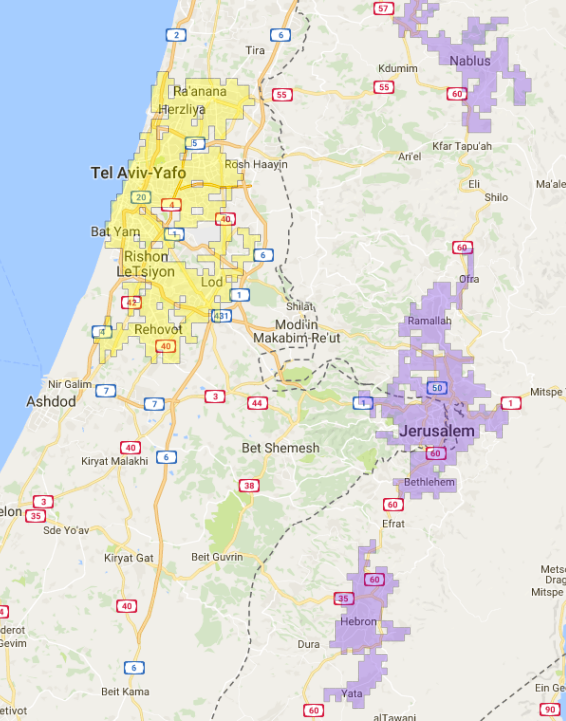
\includegraphics[width=\textwidth]{TelAviv}
  \caption{Geographic Definition of Tel Aviv-Yafo}
   \label{fig:TelAviv}
\end{centering}
\end{figure}
\end{comment}

